%%%%%%%%%%%%%%%%%%%%%%%%%%%%%%%%%%%%%%%%%
% University/School Laboratory Report
% LaTeX Template
% Version 3.1 (25/3/14)
%
% This template has been downloaded from:
% http://www.LaTeXTemplates.com
%
% Original author:
% Linux and Unix Users Group at Virginia Tech Wiki 
% (https://vtluug.org/wiki/Example_LaTeX_chem_lab_report)
%
% License:
% CC BY-NC-SA 3.0 (http://creativecommons.org/licenses/by-nc-sa/3.0/)
%
%%%%%%%%%%%%%%%%%%%%%%%%%%%%%%%%%%%%%%%%%

%----------------------------------------------------------------------------------------
%	PACKAGES AND DOCUMENT CONFIGURATIONS
%----------------------------------------------------------------------------------------

\documentclass{article}

\usepackage[version=3]{mhchem} % Package for chemical equation typesetting
\usepackage{siunitx} % Provides the \SI{}{} and \si{} command for typesetting SI units
\usepackage{graphicx} % Required for the inclusion of images
\usepackage{natbib} % Required to change bibliography style to APA
\usepackage{amsmath} % Required for some math elements 
\usepackage{enumerate} % Required for the enumerate function
\usepackage[americanvoltages,siunitx]{circuitikz} % Required for the drawing of circuit diagrams
\usepackage{caption}
\usepackage{graphicx}
\usepackage{subcaption}
\usepackage{xfrac}
\usepackage{float}
\usepackage{enumitem}
\usepackage{epstopdf}
\usepackage{booktabs}
\usepackage[]{mcode}
\usepackage{tikz}
\usetikzlibrary{shapes,arrows}
\usepackage{verbatim}
\usepackage{textcomp}
\usepackage{mathrsfs}

\setlength\parindent{0pt} % Removes all indentation from paragraphs

\renewcommand{\labelenumi}{\alph{enumi}.} % Make numbering in the enumerate environment by letter rather than number (e.g. section 6)

%\usepackage{times} % Uncomment to use the Times New Roman font

\graphicspath{{./fig/}}

%----------------------------------------------------------------------------------------
%	DOCUMENT INFORMATION
%----------------------------------------------------------------------------------------

\title{Systems Modelling \& Control \\ Lab 2 \\ ENG325} % Title

\author{Shane \textsc{Reynolds}} % Author name

\date{\today} % Date for the report

\begin{document}

\maketitle % Insert the title, author and date

\begin{center}
\begin{tabular}{l r}
Date Performed: & March 25, 2016 \\ % Date the experiment was performed
Instructor: & Damien Hill % Instructor/supervisor
\end{tabular}
\end{center}

% If you wish to include an abstract, uncomment the lines below
% \begin{abstract}
% Abstract text
% \end{abstract}

%----------------------------------------------------------------------------------------
%	SECTION 1
%----------------------------------------------------------------------------------------

\section{Objective}

To model a pump tank system by recording the frequency response to a frequency sweep on the input signal, and provide discussion with respect to model accuracy when compared to a model derived in the time domain.

\section{Background}

The pump tank system is illustrated in Figure 1. The input voltage to the pump is denoted by $u(t)$, and can be thought of as acting as a proxy for pump speed, or flow rate into the tank. The output signal, $y(t)$, is the voltage from a sensor in the tank which provides a measurement of the height of the water in the tank column. When in operation the system is at a steady state for some given DC input voltage $\bar{u}(t)$. On top of the DC signal, $\bar{u}(t)$, a sinusoidal signal is superimposed, $\tilde{u}(t)$.

% Draw a simple picture of the pump tank system use this section to calculate the cross sectional area of the device.
\tikzstyle{block} = [draw, fill=blue!20, rectangle, 
minimum height=3em, minimum width=6em]
\tikzstyle{sum} = [draw, fill=blue!20, circle, node distance=1cm]
\tikzstyle{input} = [coordinate]
\tikzstyle{output} = [coordinate]
\tikzstyle{pinstyle} = [pin edge={to-,thin,black}]

% The block diagram code is probably more verbose than necessary
\begin{figure}[H]
	\centering
	\caption{Pump Tank Fluid System}
	\begin{tikzpicture}[auto, node distance=2cm,>=latex']
	% We start by placing the blocks
	\node [block, name=pump, pin={[pinstyle,pin edge={<-}]above:$u(t)$}]{Pump};
	\node [block, right of=pump, node distance=3cm, pin={[pinstyle,pin edge={->}]above:$y(t)$}](tank){Tank};
	\draw[->] (pump) -- node [name=u] {} (tank);
	\node [block, below of=u] (reservoir){Reservoir};
	\node [name=t, right of=tank]{};
	\node [name=v, below of=t]{};
	\draw[->] (tank) -- node [name=z] {}(tank-|v) |- (reservoir);
	\node [name=a, left of=pump]{};
	\draw[->] (reservoir) -- (reservoir -| a) |- (pump);
	\end{tikzpicture}
\end{figure}

%----------------------------------------------------------------------------------------
%	SECTION 2
%----------------------------------------------------------------------------------------

\section{Data Acquisition}

As outlined above, the voltage input, $u(t)$, consists of a DC input, $\bar{u}(t)$, and a variable sinusoidal signal, $\tilde{u}(t)$, and can be written as:
\begin{align*}
	u(t) = \bar{u}(t) + \tilde{u}(t)
\end{align*}

The DC input, $\bar{u}(t)$, was selected such that the water level in the tank is at approximately 50\% of the tank volume. The small signal, is a sinusoid, which in general can be denoted as:
\begin{align*}
	\tilde{u}(t) = A \sin(\omega t + \theta)
\end{align*}

The amplitude of $\tilde{u}(t)$, $A$, was set such that the water level does not drop below 20\%, or reach above 80\%, of the total tank volume. Data for both the input, $u(t)$, and the output, $y(t)$, was collected for the following frequency values, $\omega$, of the input signal: 0.05$\si{\radian\per\second}$, 0.1 $\si{\radian\per\second}$, 0.2 $\si{\radian\per\second}$, 0.5 $\si{\radian\per\second}$, 1.0 $\si{\radian\per\second}$, 2.0 $\si{\radian\per\second}$, 5.0 $\si{\radian\per\second}$, and 10.0 $\si{\radian\per\second}$.


%----------------------------------------------------------------------------------------
%	SECTION 3
%----------------------------------------------------------------------------------------

\section{MATLAB Analysis}

The plot in Figure 2 shows the input signal, $u(t)$, and the output signal, $y(t)$, plotted against time for each frequency. The input signal, $u(t)$, for some frequency, $\omega$, can be written as follows:
\begin{align*}
	u(t) = \bar{u}(t) + A \sin(\omega t + \theta)
\end{align*}

Similarly, given a frequency, $\omega$, the output, $y(t)$, can be modelled as:
\begin{align*}
	y(t) = \bar{y}(t) + B \sin(\omega t + \phi)
\end{align*}

It is difficult to fully specify the models using a parameter estimation technique like linear regression since the phase parameters, $\theta$ and $\phi$, provide for an infinite number of curves, which could lead to drastically misspecified phase lag between the input and output. This does not mean that linear regression can not help - fitting sinusoidal curves allows for the correct specification of the amplitude parameters, $A$ and $B$, for the input and output signals, respectively. Further, the DC components of the input and output signals were also found.\\

The results of the parameter estimation from linear regression methods can be seen in Table 1. Kamen and Heck (2007) state that the output of a system, $y(t)$, in the time domain can be found by taking the convolution of the impulse response, $h(t)$, and the input signal $u(t)$, that is:

\begin{align}
	y(t) = h(t)*u(t)
\end{align}

\begin{figure}[H]
	\hspace*{-4.2cm}
	\centering
	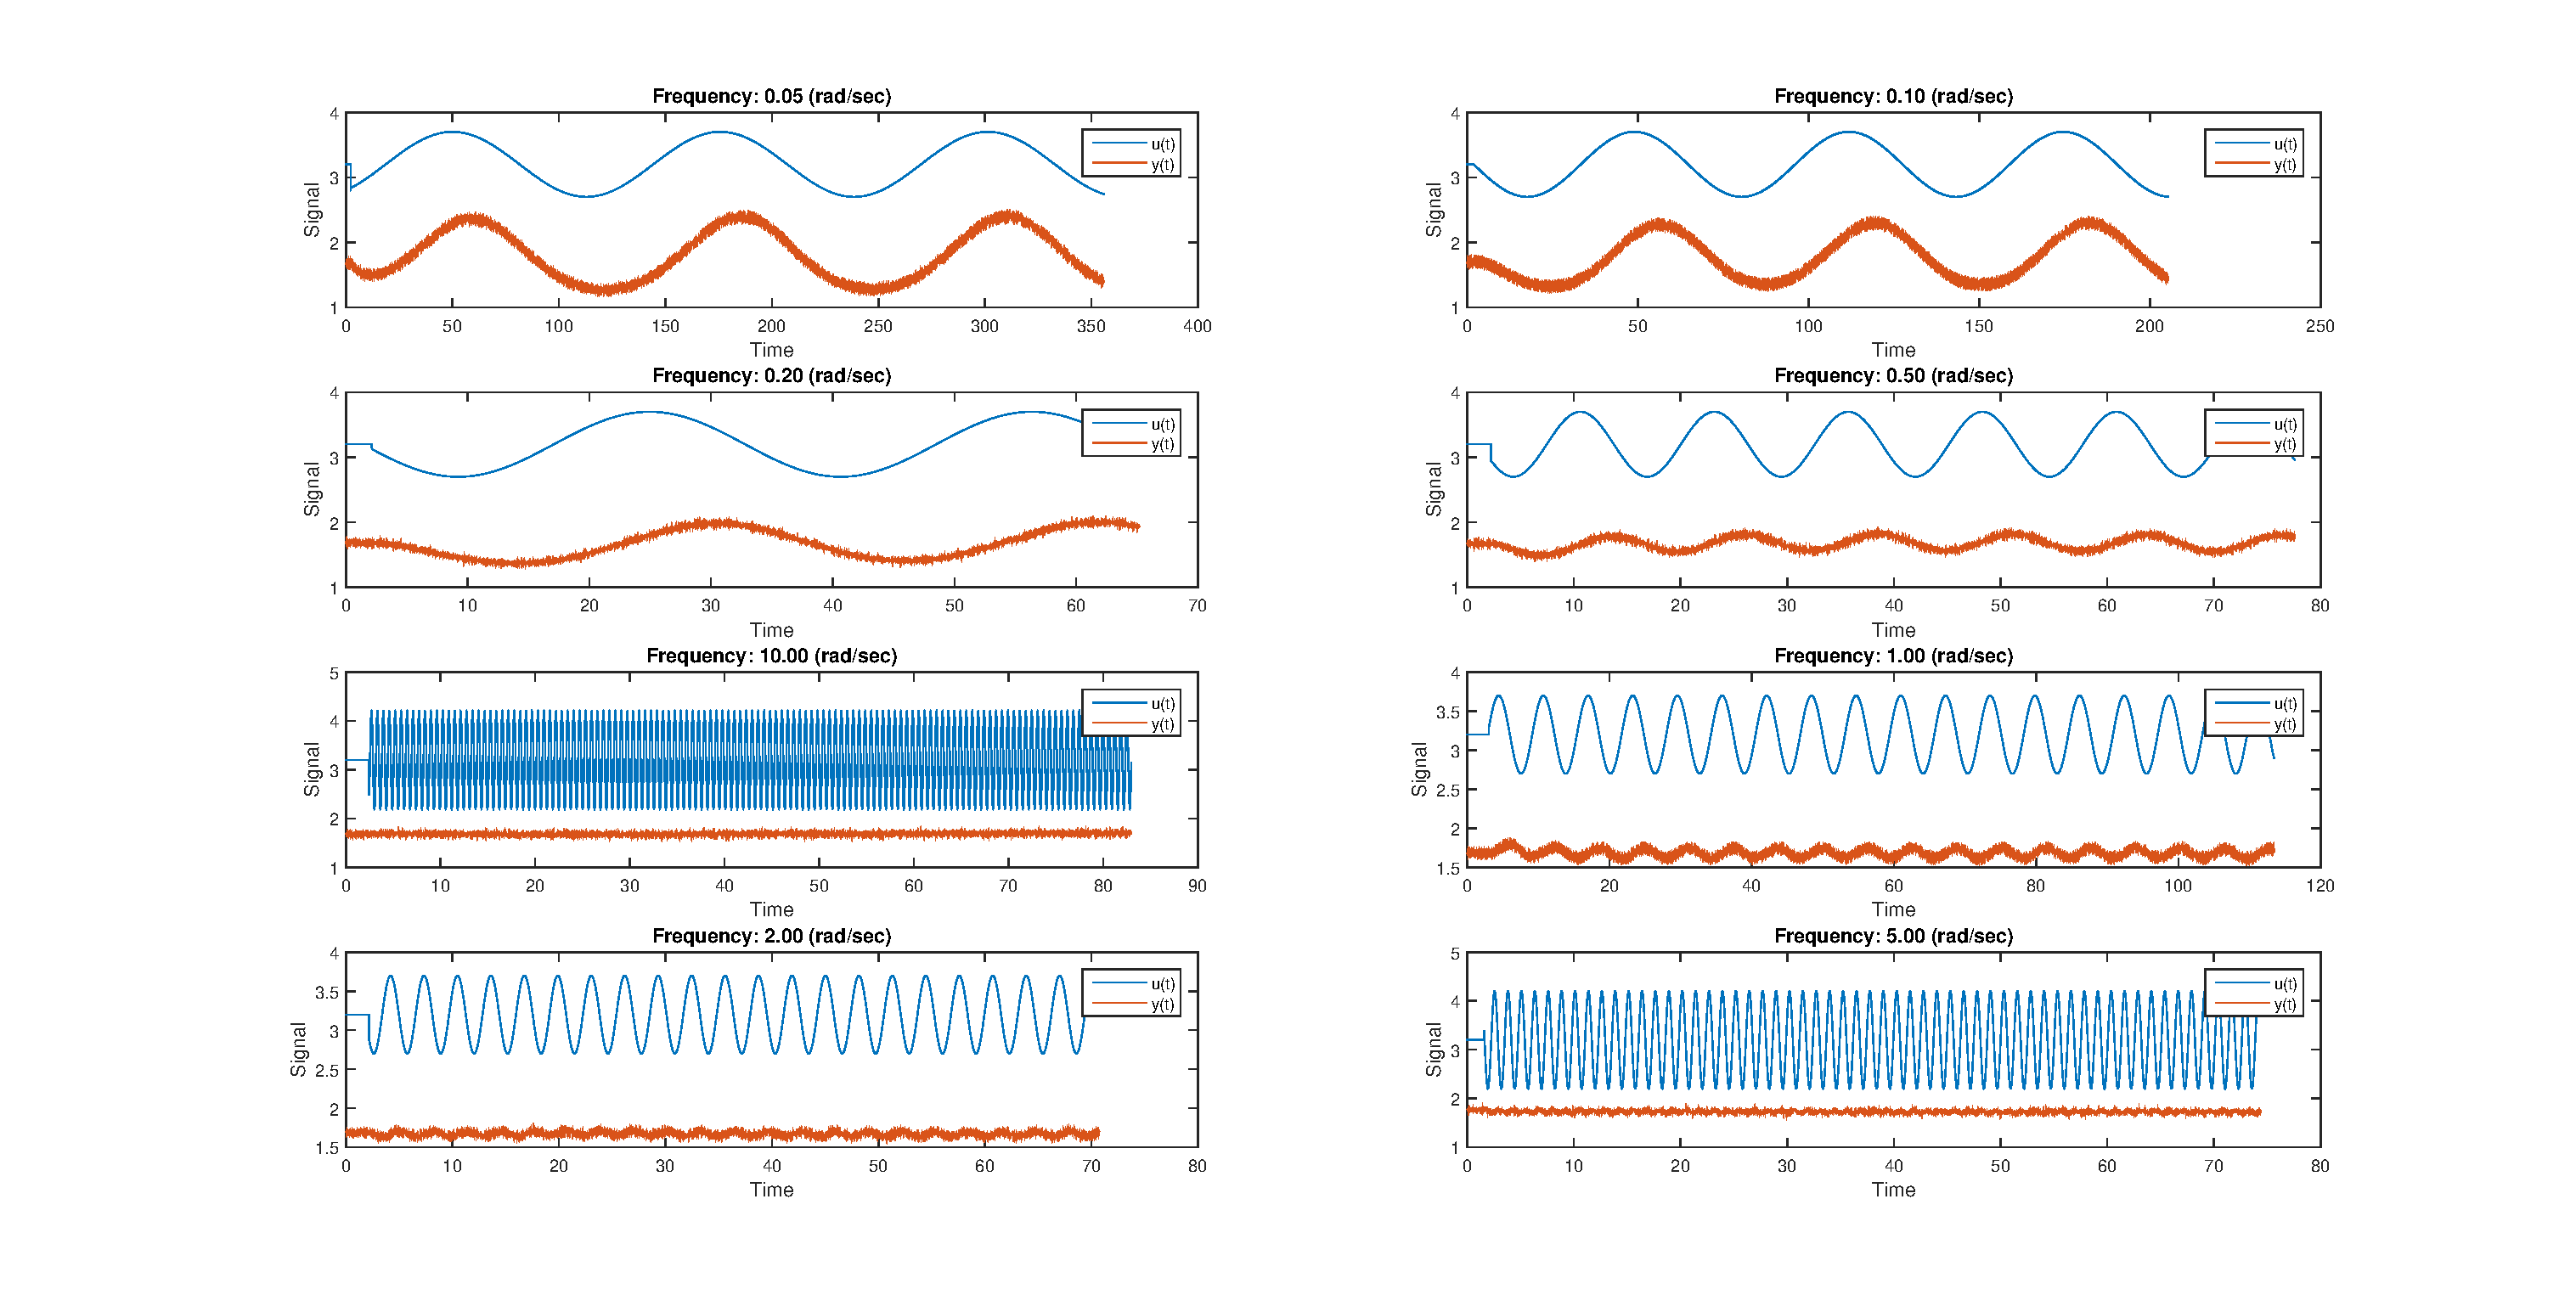
\includegraphics[scale=0.4]{fig1.eps}
	\captionof{figure}{Time series plot of input and output signal}
\end{figure}

Of course an impulse is difficult, if not impossible, to generate in real life. Taking the Fourier transform of both sides of equation (1) yields:
\begin{align*}
	\mathscr{F}\{y(t)\} &= \mathscr{F}\{h(t)*u(t)\}\\
	Y(j\omega) &= H(j\omega)U(j\omega)
\end{align*}

Rearranging allows us to find an expression for the transfer function, $H(\omega)$, in terms of $Y(\omega)$ and $X(\omega)$, that is:
\begin{align*}
	H(j\omega) = \frac{Y(j\omega)}{X(j\omega)}
\end{align*}

The magnitude of the transfer function is given by:
\begin{align*}
	|H(j\omega)| = \frac{|Y(j\omega)|}{|X(j\omega)|}
\end{align*}

The values for both $|Y(j\omega)|$ and $|X(j\omega)|$ are simply the amplitude of the output signal and input signal, $B$ and $A$, which were estimated earlier. The calculated values for $|H(\omega)|$ can be found in Table 1.

\begin{table}[H]
	\centering
	\caption{Experimental data from frequency sweep on input signal}
	\begin{tabular}{S[table-format=3.2] S[table-format=3.2] S[table-format=3.2] S[table-format=3.2] S[table-format=3.2] S[table-format=3.2]}
		\toprule
		{$\omega$}  & {$\bar{u}(t)$} & {$A$} & {$B$} & {$|H(j \omega)|$} & {$\angle H(j \omega)$}\\
		{($\si{\radian\per\second}$)} & {($\si{\volt}$)} & {($\si{\volt}$)} & {($\si{\volt}$)} & {($\si{\decibel}$)} & {($\si{\deg}$)} \\\midrule
		0.05 & 3.2027 & 0.4956 & 0.5387 & 1.08 & -22.34\\
		0.10 & 3.1996 & 0.4998 & 0.4651 & 0.93 & -40.22\\
		0.20 & 3.1990 & 0.4993 & 0.2831 & 0.56 & -56.95\\
		0.50 & 3.1996 & 0.4971 & 0.1234 & 0.24 & -80.50\\
		10.00 & 3.1996 & 0.9701 & 0.0137 & 0.01 & -143.23\\
		1.00 & 3.2085 & 0.4862 & 0.0609 & 0.12 & -91.67\\
		2.00 & 3.1942 & 0.4881 & 0.0287 & 0.05 & -103.13\\
		5.00 & 3.1968 & 0.9778 & 0.0240 & 0.02 & -123.18\\\bottomrule
	\end{tabular}
\end{table}

Finally, the phase lag, $\angle H(j\omega)$, was found using a cross correlation approach. The estimated phase lag for each frequency input can be seen in Table 1. The Matlab script which implements all of the aforementioned estimation techniques can be found in Appendix A, and the MATLAB output can be found in Appendix B. 



%----------------------------------------------------------------------------------------
%	SECTION 3
%----------------------------------------------------------------------------------------

\section{Bode Plot of Results}

The results from Table 1 were plotted in a Bode plot, which can be seen in Figure 3. The MATLAB code implementing this can be found in Appendix A.

\begin{figure}[H]
	\centering
	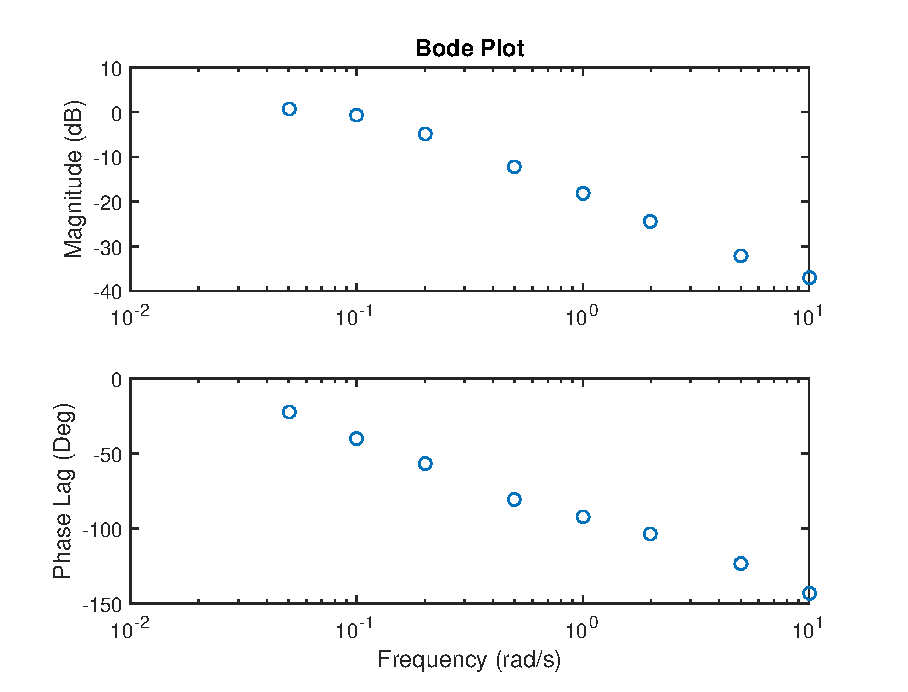
\includegraphics[scale=0.7]{fig2.eps}
	\captionof{figure}{Bode plot of transfer function}
\end{figure}

%----------------------------------------------------------------------------------------
%	SECTION 4
%----------------------------------------------------------------------------------------

\section{System Identification in Frequency Domain}

A computational approach was used to perform the system identification. Calculated values for the transfer function magnitude, $|H(j\omega)|$, and phase lag, $\angle H(j\omega)$, were transformed into a vector of complex exponentials. Using this vector as input into MATLAB, along with the 0.01 second sampling time interval, a first order transfer function was estimated with a reported fit of 94.17\%. The reported transfer function was:
\begin{align}
	H(j\omega) = \frac{0.139}{j\omega \times 0.1178}
\end{align}

Implementation of the MATLAB code can be found in Appendix A, and output from MATLAB transfer function estimation can be found in Appendix B.
%----------------------------------------------------------------------------------------
%	SECTION 5
%----------------------------------------------------------------------------------------

\section{Comparison of Models Derived in Frequency Domain and Time Domain}

The original derivation of the pump tank system in the time domain yielded a first order differential equation:
\begin{align}
	\frac{d}{dt}\big(dH(t)\big) = \frac{1}{C}dQ_i - \frac{1}{R_tC}dH(t)
\end{align}

The incremental change in the height of the water in the tank is given by $dH(t)$ in equation (3). Further, $dQ_i$ represents the incremental rate of flow into the tank. Finally, the capacitance, $C$, is the cross sectional area of the column tank, and the resistance, $R_t$, is the resistance that fluid flowing into the tank experiences. Experimental values for both $R_t$ and $C$ were found in laboratory 1. Laboratory 1 also specified the linear relationship between the height of the fluid in the tank, $H(t)$, and the voltage from the sensor, $HU(t)$, which measured the height of the water in the tank. This is given by equation (4):
\begin{align}
	HU(t) = 0.0155H(t) + 0.589
\end{align}

Further, a relationship between the input voltage to the pump, $U(t)$, and the inflow to the tank, $Q_i$, was found:
\begin{align}
	Q_i(t) = 2012.71U(t) + 589.42
\end{align}

Taking the differential of both equation (4) and (5), gives us:
\begin{align*}
	dHU(t) &= 0.0155dH(t)\\
	dQ_i(t) &= 2012.71dU(t)
\end{align*}

\newpage

Noting that we have respecified $dHU(t)$ as $y(t)$ and $dU(t)$ as $u(t)$, we can rewrite the differentials $dHU(t)$ and $dQ_i(t)$ as shown in equations (6) and (7), respectively:
\begin{align}
	y(t) &= 0.0155H(t)\\
	dQ_i(t) &= 	2012.71u(t)
\end{align}

Substituting equations (6) and (7) into equation (3) provides that:
\begin{align*}
	\frac{d}{dt}\bigg(\frac{y(t)}{0.0155}\bigg) = \frac{1}{C} \cdot 2012.71 \cdot u(t) - \frac{1}{R_tC} \cdot \frac{y(t)}{0.0155}
\end{align*}

Hence, we get that:
\begin{align}
\frac{d}{dt}\big(y(t)\big) = \frac{1}{C} \cdot 31.197 \cdot u(t) - \frac{1}{R_tC} \cdot y(t)
\end{align}

Now, to find the transfer function of our time domain model, we take the Laplace transform of equation (8), which we write as:
\begin{align*}
	\mathscr{L}\bigg\{ \frac{d}{dt}\big(y(t)\big) \bigg\} = \mathscr{L} \bigg\{ \frac{1}{C} \cdot 31.197 \cdot u(t) - \frac{1}{R_tC} \cdot y(t)  \bigg\}
\end{align*}

This gives us:
\begin{align*}
	sY(s) = 31.197 \cdot \frac{1}{C} \cdot X(s) - \frac{1}{R_tC} \cdot Y(s)
\end{align*}

Rearranging, we obtain the transfer function:
\begin{align}
	H(s) = \frac{Y(s)}{X(s)} = \frac{31.197 \cdot \frac{1}{C}}{s + \frac{1}{R_tC}}
\end{align}

In laboratory 1, $R_t$ and $C$ were determined using experimental data at the 50\% DC bias level such that $R_t = 0.0305$ $\si{\second\per\milli\meter^2}$ and $C = 258.76$ $\si{\milli\meter^2}$. Hence we can specify equation (9) as:
\begin{align*}
	H(s) = \frac{0.121}{s + 0.1267}
\end{align*}

Finally, given that $s = \sigma + j\omega$ we can say that $s = j\omega$ provided that the region of convergence for $X(\omega)$ includes $\sigma = 0$ (Kammen and Heck, 2007). If this condition holds we can conclude that:
\begin{align}
	H(j \omega) = \frac{0.121}{j \omega + 0.1267}
\end{align}

A comparison of the magnitude of the transfer function, $|H(j\omega)|$, for the time domain derivation, the frequency domain derivation, and the captured experimental data can be seen in Figure 4. The figure shows that the experimental data closely follows the model derived from the system identification. This is to be expected as software was used to fit the model to the experimental data. Since this model has been derived experimentally it will carry some bounded measurement error, which is inherent in the voltage measurement devices. It must be noted, however, that the model derived in the time domain would also carry some measurement errors from the estimated model parameters, $R_t$ and $C$, and from the estimated equations which link the model input and output, $Q_i(t)$ and $H(t)$, to observable variables, $U(t)$ and $HU(t)$, respectively.\\

\begin{figure}[H]
	\centering
	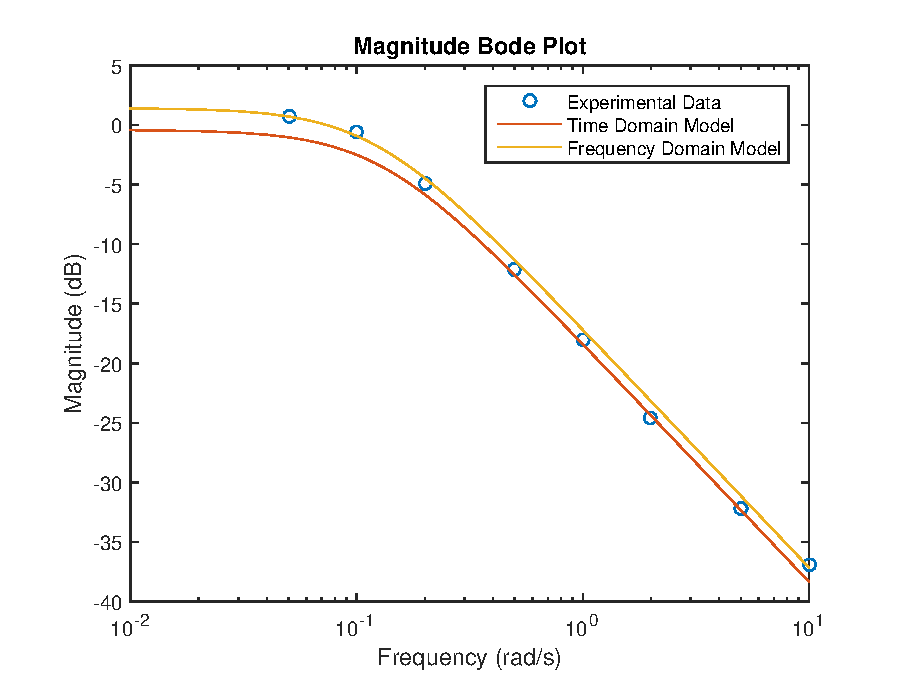
\includegraphics[scale=0.7]{fig3.eps}
	\captionof{figure}{Comparison of the magnitude of the transfer function versus frequency for the model derived in the time domain, the frequency domain, and the captured data}
\end{figure} 

Additionally, both models carry error due to linearisation. The frequency domain model was derived under the assumption that the underlying system was linear, and it was seen in laboratory 1 that to obtain our time domain differential equation, we relied on linearising non-linear system elements. The point worth highlighting is that both models carry error due to measurement, and due to a linearisation assumption. It is therefore reasonable to assume that both models deviate from the true underlying model by a statistically similar amount. Moreover, the principal reason for the observable differences in the two models can be attributed to the fact that different experimental data sets were used derive each model - it must be stressed, however, that these model differences are only marginal. Furthermore, important model features, such as the slope of the curve for higher frequencies, are almost identical. This leads to the conclusion that both models yield similar accuracy in their estimation of the true underlying system. Evidence supporting this conclusion can be seen in the closely matching phase plots in seen in Figure 5.

\begin{figure}[H]
	\centering
	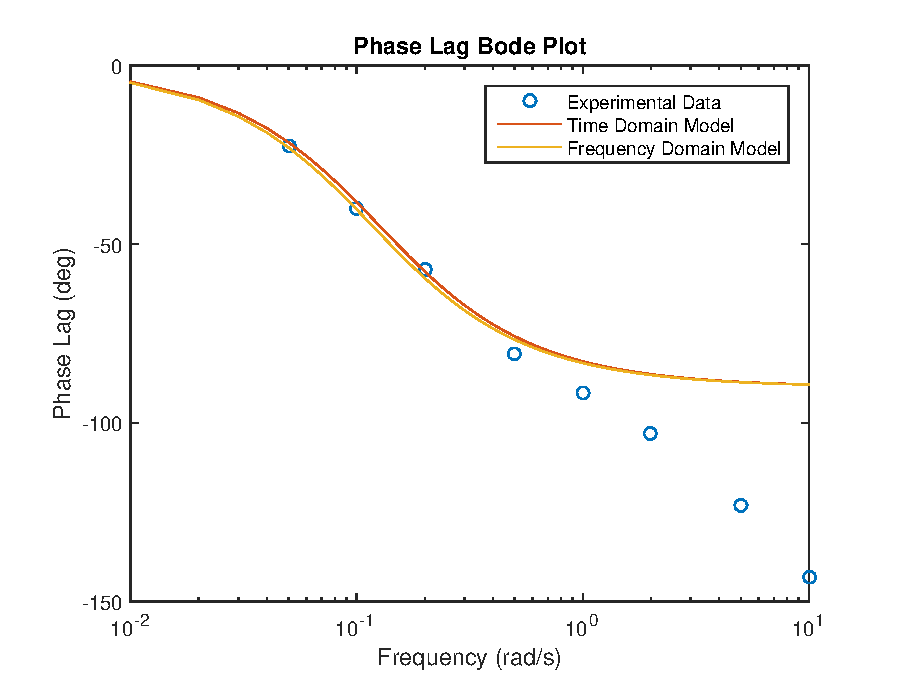
\includegraphics[scale=0.7]{fig4.eps}
	\captionof{figure}{Comparison of the phase lag of the transfer function versus frequency for the model derived in the time domain, the frequency domain, and the captured data}
\end{figure}

Finally, worth mentioning is the striking divergence of the experimental data from the derived models, seen in Figure 5. This divergence is too large to be attributed to measurement error, and warrants further exploration. Most likely the divergence is due to an error in the estimation of the phase lag using a cross correlation technique. Interestingly, the derivation of the frequency domain model relied on these divergent phase lag estimates, which may be an explanation why only 94\% of the variation in the experimental data was being explained by the model. Perhaps if correct estimates were obtained for the phase lag, we would see system identification closer to 100\%.

\newpage

\section{Relevance of Laboratory Assignment}
I think these pump tank labs have been really well designed - they provide an opportunity for an open ended investigation and probide opportunity to go into higher technical detail if desired. I've really enjoyed myself with this and it's allowed me to tie together several of my courses from my Applied Mathematics degree. The only point of improvement is perhaps providing guidance on how to discover the phase lag between two signals. I have spent considerable time on this problem, first in Analog Circuits, and then in Circuit Analysis, and now in Systems Modelling. I understand that it can be observed and found by hand, but this seems like a crude method. I have tried using the Fast Fourier Transform to do this, and also a cross correlation method that I found on Stack Exchange, but both have resulted in error, from what I can see. I am still unsure as to how you would do this effectively, or if you would ever actually need these values.

%----------------------------------------------------------------------------------------
%	BIBLIOGRAPHY
%----------------------------------------------------------------------------------------

\section{References}
Kammen, E. W., \& Heck, B. S. (2007). \textit{Fundamentals of Signals and Systems Using the Web and MATLAB 3rd Edn}. Pearson.

\newpage

%----------------------------------------------------------------------------------------
%	APPENDIX
%----------------------------------------------------------------------------------------

\section{Appendices}

\subsection{Appendix A}
Implementation of simulation using Matlab:
\begin{lstlisting}
	%%%%%%%%%%%%%%%%%%%%%%%%%%%%%%%%%%%%%%%%%%%%%%%%%%%%%%%%%%%%%%%%%%%%%%%%%%%%%
	% Script takes a series of files, extracts data, plots input and output
	% signals for the system and runs linear regression to determine amplitudes
	% and cross correlation to determine phase lag. Further, script creates
	% Bode plot for data and then estimates Transfer function for system.
	%%%%%%%%%%%%%%%%%%%%%%%%%%%%%%%%%%%%%%%%%%%%%%%%%%%%%%%%%%%%%%%%%%%%%%%%%%%%%
	
	clc; clear;
	% Create a general path string that can use used to access file paths
	path_name = 'C:\Users\Shane Reynolds\Desktop\ENG325 Lab 2 data\ENG325 Lab 2 data\';	
	% Create a general tag to build .txt file list
	gen_path = '*.txt';
	% Store file list in files
	files = dir(strcat(path_name,gen_path));
	% Frequencies used in experiment
	frequency = [0.05 0.1 0.2 0.5 10.0 1.0 2.0 5.0];
	L = length(frequency);
	% Create storage vectors for signal parameters
	Au = zeros(1,L); ubar = zeros(1,L); Ay = zeros(1,L);
	ybar = zeros(1,L); phlag = zeros(1,L);
	
	% Loop creates a subplot which plots input and response. Also determines
	% signal amplitude, DC signal and phase lag for each file
	for i = 1:length(frequency)
		% Pull file path and load data from file into system store in data
		new_path = strcat(path_name,files(i).name);
		data = csvread(new_path);
		% t is the time for which the process was run, u is the input data,
		% and y is the output data
		t = data(:,1); u = data(:,2); y = data(:,3);
		% Determine the subplot entry to plot in
		figure(1)
		subplot(4,2,i);
		% Plot the input signal, title the graph and label the axes
		sigplot(t,u,y,frequency(i))
		% Obtain DC bias, signal amplitude and phase lag
		[Au(i), ubar(i), Ay(i), ybar(i), phlag(i)] = coeffgrab(t,u,y,frequency(i));
	end
	
	% Transfer function magnitude vector
	H_mag = abs(Ay)./abs(Au);
	% Display model parameters
	parameter_printout(frequency,ubar,Au,Ay,H_mag,phlag);
	% Create Bode plot
	figure(2);
	plot_bode(frequency, H_mag, phlag)
	% System identification of 1st order transfer function
	systidf(frequency,H_mag,phlag)
	
\end{lstlisting}

\newpage
This function obtains the parameter estimations for a given input and output:
\begin{lstlisting}
	function [Au, ubar, Ay, ybar, phlag] = coeffgrab(t,u,y,freq)
	
		% Create model type to be fitted to curves
		curve = sprintf('ubar + A*sin(%1.2f*x + theta)', freq);
		type = fittype(curve);
	
		% Discover amplitude of input signal
		fitcurve_u = fit(t,u,type);
		coeff_u = coeffvalues(fitcurve_u);
		Au = coeff_u(1);
		ubar = coeff_u(3);
	
		% Discover amplitude of output signal
		fitcurve_y = fit(t,y,type);
		coeff_y = coeffvalues(fitcurve_y);
		Ay = coeff_y(1);
		ybar = coeff_y(3);
	
		% Remove DC components from signal in preparation to use cross
		% corr
		u_nodc = u - mean(u);
		y_nodc = y - mean(y);
	
		% Phase lag discovery
		[c,lag] = xcorr(u_nodc,y_nodc);
		[maxC,idx] = max(c);
		lag = lag(idx);
		phlag = 360/(2*pi)*freq*lag*0.01;
	end
\end{lstlisting}

This function creates bode plots for the transfer function:
\begin{lstlisting}
	function plot_bode(freq, H_mag, phlag)
	
		% Convert
		dB_H_mag = mag2db(H_mag);
	
		% Plot the magnitude function
		subplot(2,1,1);
		semilogx(freq, dB_H_mag, 'o');
		title('Bode Plot');
		ylabel('Magnitude (dB)');
	
	
		% Plot the phase function
		subplot(2,1,2);
		semilogx(freq, phlag, 'o');
		xlabel('Frequency (rad/s)');
		ylabel('Phase Lag (Deg)');
	
	end
\end{lstlisting}

\vspace{1cm}
This function creates plots of the input signal and output signal in the time domain:
\begin{lstlisting}
	function sigplot(t,u,y,freq)
	
		% Plot input signal
		plot(t,u);
		hold on;
		tString = sprintf('Frequency: %1.2f (rad/sec)' ,freq);
		title(tString);
		xlabel('Time');
		ylabel('Signal');
	
		% Plot output signal
		plot(t,y);
		legend('u(t)','y(t)','Location','northeast');
	
	end
\end{lstlisting}

\vspace{1cm}
This function performs the task of system identification:
\begin{lstlisting}
	function systidf(freq,H_mag,phlag)
	
		fprintf('\n\n\nEstimating Transfer Function...\n');
	
		% Complex frequency response data of the system
		zfr = H_mag.*exp(1i*phlag*pi/180);
	
		% Time sampling intervals 
		Ts = 0.01;
	
		% Create idfrd object to pass to t/fer function discovery
		gfr = idfrd(zfr,freq,Ts);
	
		% Bode plot of idfrd object
		figure(3)
		bode(gfr);
	
		% System identification using a first order model
		tfest(gfr,1)
	end
\end{lstlisting}

\newpage
This function simply prints out the estimated parameters to the MATLAB terminal
\begin{lstlisting}
	function parameter_printout(freq,ubar,Au,Ay,H_mag,phlag)
	
		% Printout headings
		fprintf('\n\n\nEstimating parameters...\n');
		data = [ubar' Au' Ay' H_mag' phlag'];
	
		%row_name = {'ROW1','ROW2','ROW3','ROW4','ROW5','ROW6','ROW7','ROW8'};
		%col_name = {'Freq','ubar','Au','Ay','H_mag','H_Phase_lag'};
		%array2table(data, 'VariableNames', col_name, 'RowNames', row_name)
	
		row_name = ...
		'Freq(0.05) Freq(0.10) Freq(0.20) Freq(0.50) Freq(10.0) Freq(1.0) Freq(2.0) Freq(5.0)';
		col_name = 'ubar Au Ay H_mag H_Phase_lag';
		printmat(data, 'SIGNAL PARAMETERS',row_name,col_name);
		
	end
\end{lstlisting}

\newpage
This script plots comparisons of the experimental data, and transfer functions for the time domain model derivation and the frequency domain derivation:
\begin{lstlisting}
	clf;
	% Acutal data captured experimentally from the pump tank system
	frequency = [0.05 0.1 0.2 0.5 10.0 1.0 2.0 5.0];
	y_mag_data = [1.0870 0.9306 0.5670 0.2483 0.0142 0.1254 0.0589 0.0246];
	y_ph_data = [-22.3454 -40.2216 -56.9520 -80.5006 -143.2394 -91.6732 -103.1324 -123.1859];
	
	% Provide a vector of frequencies to feed to derived transfer functions
	w = linspace(0.01,10,1000);
	
	% Transfer function from the time domain derivation of the pump tank system
	y_time = 0.121./(1i.*w + 0.1267);
	
	% Transfer function from the frequency response derivation of the pump tank
	% system
	y_frequency = 0.139./(1i.*w + 0.1178);
	
	% Plot comparing the experimental data, transfer function 1 and transfer
	% function 2
	figure(1)
	semilogx(frequency, mag2db(y_mag_data),'o');
	hold on;
	semilogx(w, mag2db(abs(y_time)));
	semilogx(w, mag2db(abs(y_frequency)));
	legend('Experimental Data','Time Domain Model','Frequency Domain Model')
	xlabel('Frequency (rad/s)')
	ylabel('Magnitude (dB)')
	title('Magnitude Bode Plot')
	
	figure(2)
	semilogx(frequency, phlag, 'o');
	hold on;
	semilogx(w, angle(y_time)*180/pi);
	semilogx(w, angle(y_frequency)*180/pi);
	legend('Experimental Data','Time Domain Model','Frequency Domain Model')
	xlabel('Frequency (rad/s)')
	ylabel('Phase Lag (deg)')
	title('Phase Lag Bode Plot')
\end{lstlisting}

\newpage
\subsection{Appendix B}
MATLAB output from running main script at the start of Appendix A:

\begin{verbatim}
	Estimating parameters...
	
	SIGNAL PARAMETERS = 
	                    ubar           Au           Ay        H_mag  H_Phase_lag
	Freq(00.05)      3.20276      0.49563     -0.53875      1.08699    -22.34535
	Freq(00.10)      3.19962     -0.49983      0.46515      0.93061    -40.22164
	Freq(00.20)      3.19905     -0.49939      0.28315      0.56699    -56.95200
	Freq(00.50)      3.19967      0.49713      0.12346      0.24834    -80.50057
	Freq(10.00)      3.19961      0.97013     -0.01374      0.01417   -143.23945
	Freq(01.00)      3.20851     -0.48621     -0.06095      0.12536    -91.67325
	Freq(02.00)      3.19424      0.48815     -0.02877      0.05893   -103.13240
	Freq(05.00)      3.19688      0.97786      0.02403      0.02457   -123.18593
	
	
	
	
	Estimating Transfer Function...
	
	ans =
	
	0.139
	----------
	s + 0.1178
	
	Continuous-time identified transfer function.
	
	Parameterization:
	Number of poles: 1   Number of zeros: 0
	Number of free coefficients: 2
	Use "tfdata", "getpvec", "getcov" for parameters and their uncertainties.
	
	Status:                                                
	Estimated using TFEST on frequency response data "gfr".
	Fit to estimation data: 94.17% (simulation focus)      
	FPE: 0.0007686, MSE: 0.0006229 
\end{verbatim}
\begin{lstlisting}
	
\end{lstlisting}

%----------------------------------------------------------------------------------------


\end{document}